
\documentclass[tikz,border=8pt]{standalone}
\usepackage{amsmath}
\usepackage{xcolor}
\usetikzlibrary{arrows.meta,positioning,calc,shapes.geometric}
\definecolor{Canvas}{HTML}{FAF9F6}
\definecolor{Ivory}{HTML}{FFFFF0}
\definecolor{Divider}{HTML}{E5E5EA}
\definecolor{Gold}{HTML}{C5A059}
\definecolor{WarmGold}{HTML}{D4AF37}
\definecolor{SoftPink}{HTML}{FBEFEF}
\definecolor{Ink}{HTML}{2C2C2E}
\tikzset{decision/.style={rectangle,draw=Gold,line width=1.2pt,fill=Canvas,minimum width=1.5cm,minimum height=1cm,align=center,text=Ink},chance/.style={circle,draw=WarmGold,line width=1.2pt,fill=Ivory,minimum size=1.45cm,align=center,text=Ink},payoff/.style={regular polygon,regular polygon sides=3,shape border rotate=90,draw=Gold,line width=1.2pt,fill=SoftPink,minimum size=1.25cm,align=center,text=Ink},branch/.style={draw=Ink,line width=0.9pt,-{Latex[length=2mm]},line cap=round},chosenbranch/.style={draw=Gold,line width=1.15pt,-{Latex[length=2mm]},line cap=round},callout/.style={rectangle,rounded corners=5pt,draw=Divider,fill=Ivory,text=Ink,align=center,inner sep=6pt}}

% Asset ID: OffSpecDecisionAnalysisTikZ-004
% Source: transcripts.md, utility function theory
% Purpose: Sketch utility functions and show how smaller R increases risk aversion.
\begin{document}
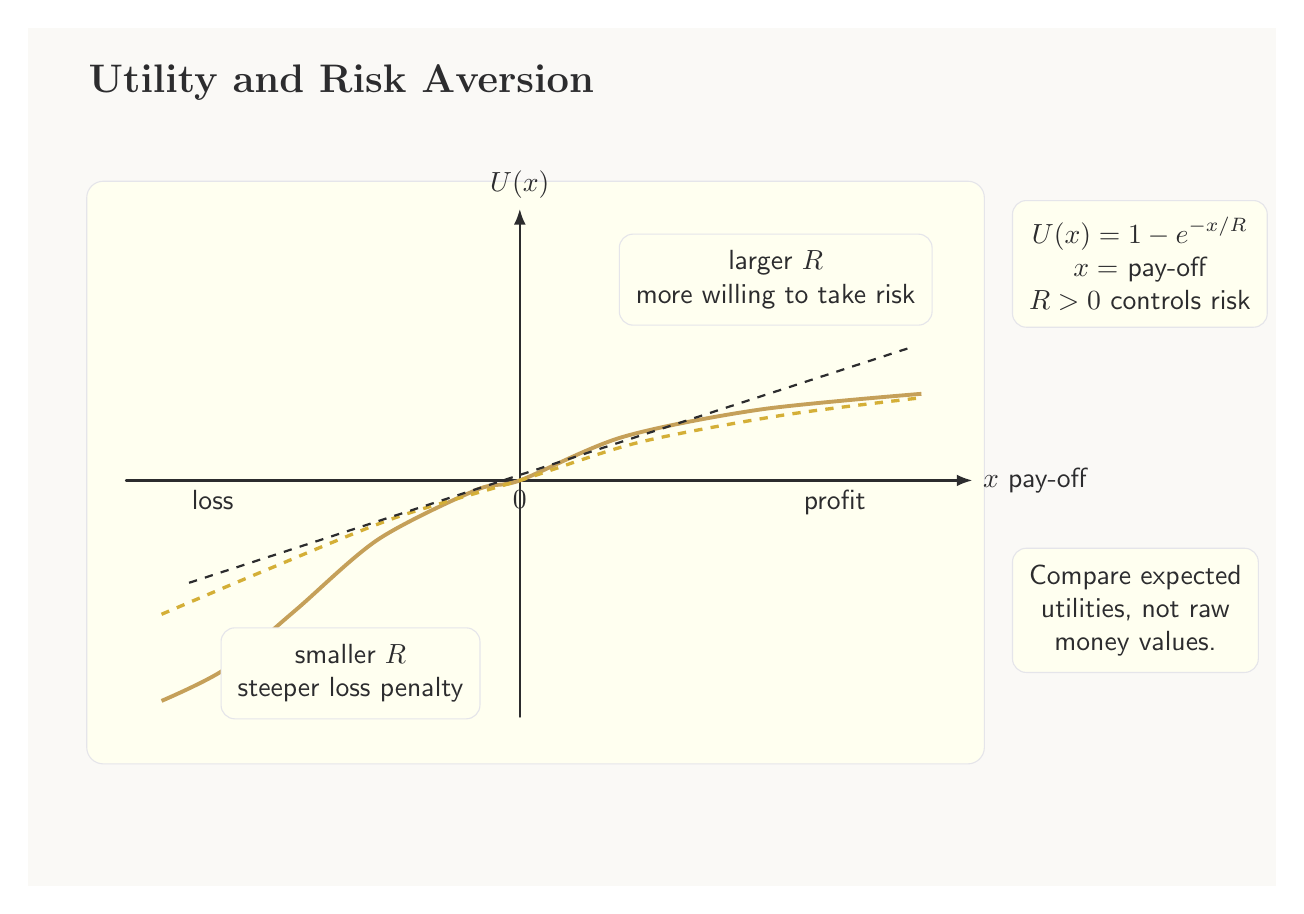
\begin{tikzpicture}[font=\sffamily,x=1cm,y=1cm]
\fill[Canvas] (-1.25,-2.15) rectangle (14.6,8.75);
\node[anchor=west,text=Ink,font=\bfseries\Large] at (-0.6,8.05) {Utility and Risk Aversion};
\fill[Ivory,draw=Divider,rounded corners=6pt] (-0.5,-0.6) rectangle (10.9,6.8);
\draw[branch] (0,3)--(10.75,3) node[right,text=Ink] {$x$ pay-off};\draw[branch] (5,0)--(5,6.45) node[above,text=Ink] {$U(x)$};
\node[text=Ink,below] at (5,3) {$0$};\node[text=Ink,below] at (1.1,3) {loss};\node[text=Ink,below] at (9.0,3) {profit};
\draw[Gold,line width=1.4pt] plot[smooth] coordinates{(0.45,0.20)(1.25,0.60)(2.15,1.35)(3.20,2.25)(4.45,2.88)(5.00,3.00)(6.30,3.55)(8.05,3.90)(10.1,4.10)};
\draw[WarmGold,line width=1.2pt,dashed] plot[smooth] coordinates{(0.45,1.30)(1.75,1.85)(3.40,2.52)(5.00,3.00)(6.50,3.48)(8.35,3.83)(10.1,4.05)};
\draw[Ink,line width=0.8pt,dashed] (0.8,1.7)--(10.0,4.7);
\node[callout] at (2.85,0.55) {smaller $R$\\steeper loss penalty};\node[callout] at (8.25,5.55) {larger $R$\\more willing to take risk};
\node[callout,anchor=west] at (11.25,5.75) {$\displaystyle U(x)=1-e^{-x/R}$\\$x=$ pay-off\\$R>0$ controls risk};
\node[callout,anchor=west] at (11.25,1.35) {Compare expected\\utilities, not raw\\money values.};
\end{tikzpicture}
\end{document}
